% CVPR-style template
\documentclass[10pt,twocolumn,letterpaper]{article}

\usepackage[pagenumbers]{cvpr}

\usepackage{subcaption}
\usepackage{graphicx}
\usepackage{amsmath}
\usepackage{amssymb}
\usepackage{booktabs}
\usepackage{array}
\usepackage[dvipsnames]{xcolor}
\usepackage{xeCJK}
\setCJKmainfont{Noto Serif CJK TC}

\usepackage[pagebackref,breaklinks,colorlinks]{hyperref}
\usepackage[capitalize]{cleveref}
\crefname{section}{Sec.}{Secs.}
\Crefname{section}{Section}{Sections}
\Crefname{table}{Table}{Tables}
\crefname{table}{Tab.}{Tabs.}

\begin{document}

\title{\LARGE HW2: Digit Detection Report \\[0.5em] \large Visual Recognition using Deep Learning, NYCU}
\author{朱驛庭, 111550093}
\maketitle

%%%%%%%%% BODY TEXT
\section{Introduction}
\label{sec:intro}

This work tackles the street-view digit detection task, a COCO-format object detection problem over 10 categories (digits 0--9). The homework mandates DETR~\cite{carion2020detr} with a ResNet-50~\cite{he2016resnet} backbone, allows modifying encoder/decoder components, and permits ImageNet pretrained weights \emph{only} for the backbone---no pretrained DETR checkpoints.

DETR casts detection as direct set prediction via a transformer encoder-decoder and bipartite matching, removing hand-crafted anchors and NMS. However, vanilla DETR suffers from slow convergence (500 epochs to match Faster R-CNN), weak small-object performance, and unstable Hungarian matching at early stages. This is catastrophic under the ``no pretrained DETR weights'' constraint: we must converge fast on limited epochs and handle small digits.

We therefore adopt \textbf{DINO}~\cite{zhang2023dino}---a state-of-the-art DETR variant---and adapt it for this task by modifying the official reference codebase\footnote{\url{https://github.com/IDEA-Research/DINO}}. DINO's three central improvements directly address our failure modes:
\begin{itemize}
  \item \textbf{Deformable multi-scale attention}~\cite{zhu2021deformable} sparsifies attention to a few learned sampling points per feature level, giving linear complexity, multi-scale features, and strong small-object recall;
  \item \textbf{Contrastive DeNoising (CDN)}~\cite{li2022dndetr,zhang2023dino} injects noised ground-truth boxes/labels as auxiliary queries, bypassing the unstable matching in the first epochs;
  \item \textbf{Mixed query selection} + \textbf{look-forward-twice} refinement further accelerate decoder convergence.
\end{itemize}

Starting from the reference code, we strip the pretrained-DETR checkpoint dependency (retaining only the ImageNet ResNet-50 backbone weights), integrate our dataset and training pipeline, disable flip augmentation (digits are not flip-invariant), and fix AMP correctness for the custom MSDeformAttn CUDA op. Under 24 epochs on 2$\times$RTX 4090, the resulting model reaches \textbf{val mAP = 0.4726} / \textbf{mAP$_{50}$ = 0.9400}, well above the strong baseline (0.38). On the CodaBench public leaderboard, our final submission scores \textbf{0.38 mAP}, placing us around \textbf{rank 30}. The remainder of the report details the method (\cref{sec:method}), results (\cref{sec:results}), and the public submission.

%------------------------------------------------------------------------
\section{Method}
\label{sec:method}

\subsection{Data Pipeline}
The provided dataset contains 30{,}062 training, 3{,}340 validation, and 13{,}068 test street-view crops in COCO format with bounding boxes for digits 0--9 (\texttt{category\_id} 1--10). All images and annotations were loaded with a custom \texttt{CocoDetection} dataset returning normalized \texttt{cxcywh} boxes.

\textbf{Augmentation.} We apply DETR-style multi-scale training: on each iteration an image is either (a) resized so the short side is sampled from $\{320,352,\ldots,640\}$ with $\max = 1024$, or (b) resized to $[400,500,600]$, random-cropped to $[384,600]^2$, then resized again. We \emph{explicitly disable horizontal flip}, because digits are not flip-invariant (e.g., $6 \leftrightarrow 9$, $2 \leftrightarrow 5$, $3 \leftrightarrow \text{mirror-3}$); flipping would inject label-inconsistent gradients. Normalization uses ImageNet mean/std.

\subsection{Architecture}
Our DINO-4-scale model (47.41 M parameters) follows~\cite{zhang2023dino}.

\textbf{Backbone.} ResNet-50~\cite{he2016resnet} with ImageNet pretrained weights (the only pretrained weights used). Feature maps from stages C3, C4, C5 plus a stride-64 projection form 4 scales, each projected to 256 channels.

\textbf{Deformable transformer encoder.} 6 layers. Each layer contains multi-scale deformable self-attention (8 heads, 4 sampling points per head per level) over the concatenated 4-scale feature tokens, plus an FFN of hidden size 2048. The sparsity of deformable attention keeps encoder cost linear in the number of tokens, enabling high-resolution feature maps critical for small digits.

\textbf{Query selection.} Encoder outputs are projected through a shared classification head; the top-900 proposals (by objectness) are selected as initial decoder positional queries (\emph{mixed query selection}---positional queries come from the encoder, content queries remain learnable). An auxiliary two-stage box head regresses proposal boxes from encoder features.

\textbf{Decoder.} 6 layers of (deformable cross-attention $\to$ self-attention $\to$ FFN). Boxes are refined layer-by-layer with \emph{look-forward-twice}: layer $l$ gradients flow through both the box it refines and the next layer's prediction, tightening the refinement chain.

\textbf{MS-Deformable attention CUDA op.} We use the MSDeformAttn CUDA kernel from the reference implementation and wrap it with \texttt{torch.cuda.amp.custom\_fwd/custom\_bwd} so it runs correctly under bf16 autocast---a subtle but essential fix we added for AMP training.

\subsection{Contrastive DeNoising (CDN)}
We add 100 denoising queries in two groups (positive/negative). For each GT box we generate noised copies:
\begin{align*}
  \tilde{b} &= b + \epsilon_b, \quad \epsilon_b \sim \mathcal{U}(-\lambda_b \cdot wh, \lambda_b \cdot wh),\\
  \tilde{c} &= c \text{ w.p. } 1-\lambda_c \text{ else random class},
\end{align*}
with $\lambda_b = 0.4$, $\lambda_c = 0.5$. Positive queries use smaller noise and must recover the original label/box; negatives use $2\times$ noise and must predict ``no object''. An attention mask blocks denoising queries from seeing matching queries and vice-versa. CDN drastically shortens the ``matching-warmup'' phase of training.

\subsection{Losses and Matching}
We use Hungarian matching with cost
$\mathcal{C} = 2\,\mathcal{C}_{\text{cls}} + 5\,\mathcal{C}_{\text{L1}} + 2\,\mathcal{C}_{\text{GIoU}}$,
where $\mathcal{C}_{\text{cls}}$ is focal-loss-based classification cost. The training loss on matched pairs is
$\mathcal{L} = 1 \cdot \mathcal{L}_{\text{focal}}(\alpha{=}0.25,\gamma{=}2) + 5 \cdot \mathcal{L}_{\text{L1}} + 2 \cdot \mathcal{L}_{\text{GIoU}}$~\cite{lin2017focal,rezatofighi2019giou}, applied to every decoder layer plus the two-stage encoder proposal (deep supervision). CDN queries use the same loss against their noised GTs.

\subsection{Optimization}
AdamW~\cite{loshchilov2019adamw}, $\text{lr}=1\mathrm{e}{-4}$ for transformer/head, $1\mathrm{e}{-5}$ for backbone, weight decay $1\mathrm{e}{-4}$, gradient clipping at $0.1$. StepLR drops $\times 0.1$ at epoch 20 of 24 total. We train in bfloat16 mixed precision on 2$\times$RTX 4090 via PyTorch DDP, batch size 6 per GPU (effective 12). Training completes in $\approx 8$ hours.

All training/validation metrics and system telemetry are logged to Weights \& Biases under project \texttt{vrdl-hw2}.

%------------------------------------------------------------------------
\section{Results}
\label{sec:results}

\subsection{Training Curves}

\cref{fig:train_loss,fig:grad_norm} show training-side dynamics. The loss decreases smoothly; the gradient norm stays bounded thanks to clipping and the AMP \texttt{custom\_fwd/bwd} wrapping of MSDeformAttn.

\begin{figure}[t]
  \centering
  
\includegraphics[width=\linewidth]{assets/train_loss.png}
  \caption{Training loss on project \texttt{vrdl-hw2}.}
  \label{fig:train_loss}
\end{figure}

\begin{figure}[t]
  \centering
  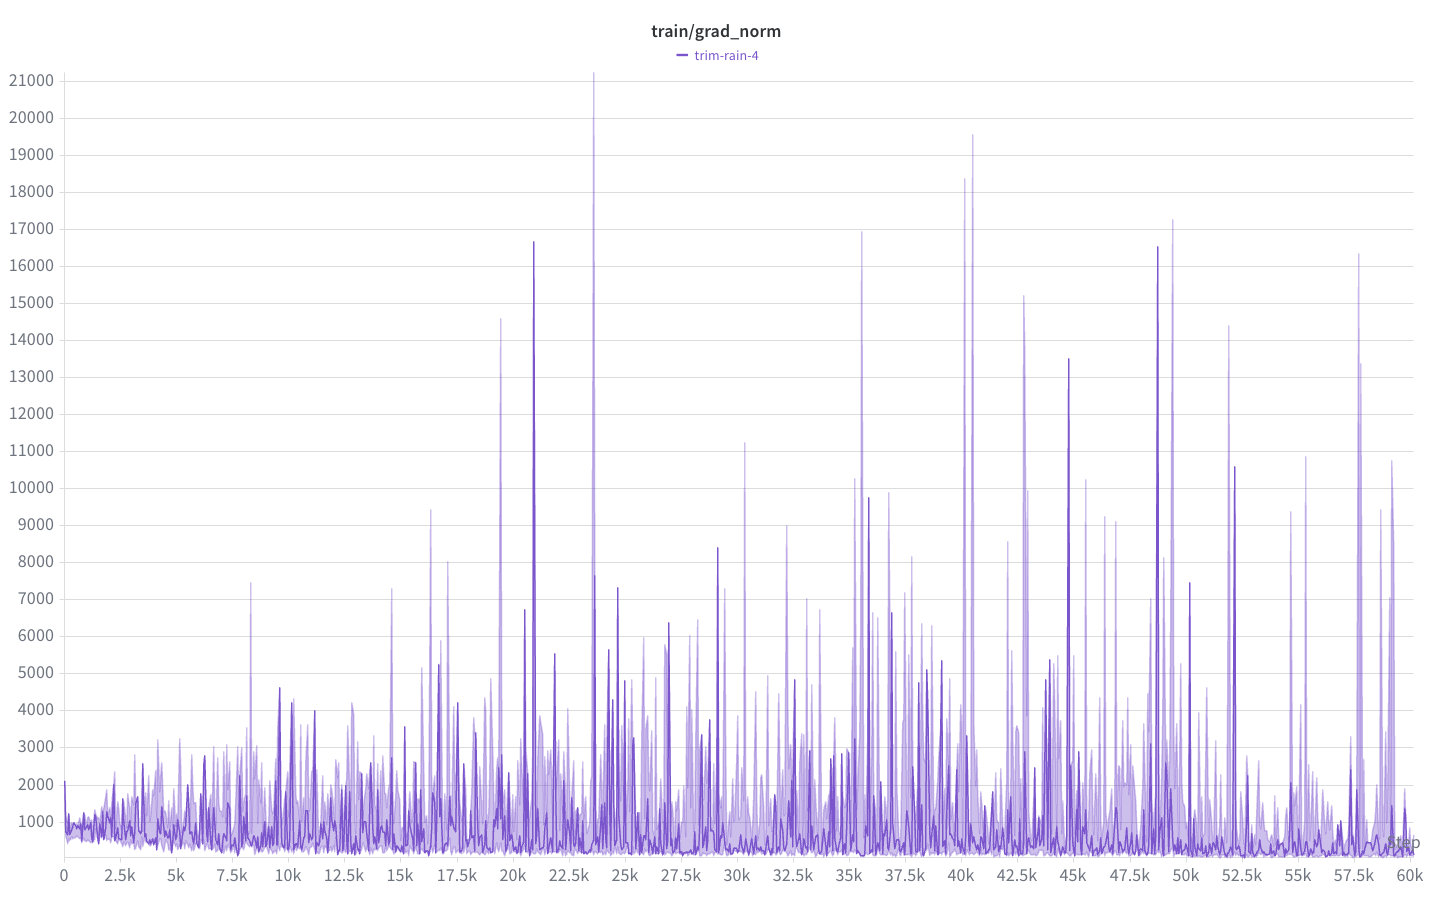
\includegraphics[width=\linewidth]{assets/train_grad_norm.png}
  \caption{Gradient norm. Stable throughout; no spikes after the AMP fix.}
  \label{fig:grad_norm}
\end{figure}

\cref{fig:val_map,fig:val_map50} show validation COCO mAP@[0.5:0.95] and mAP@0.5. Both climb rapidly (small-object-friendly deformable attention + CDN), and a clear bump appears at epoch 20 when the learning rate drops.

\begin{figure}[t]
  \centering
  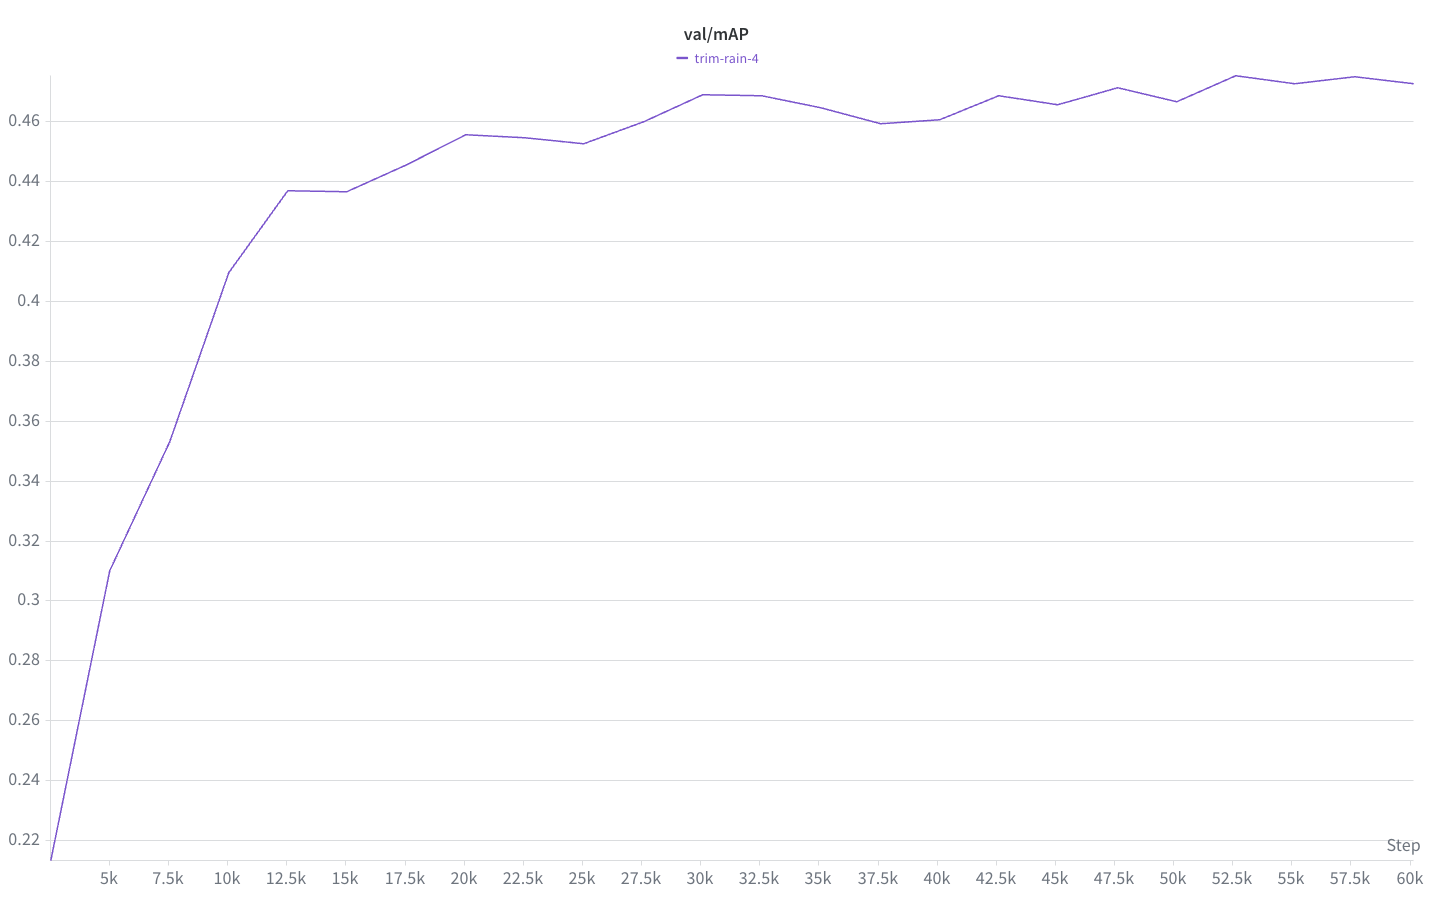
\includegraphics[width=\linewidth]{assets/val_map.png}
  \caption{Validation mAP@[0.5:0.95] over 24 epochs.}
  \label{fig:val_map}
\end{figure}

\begin{figure}[t]
  \centering
  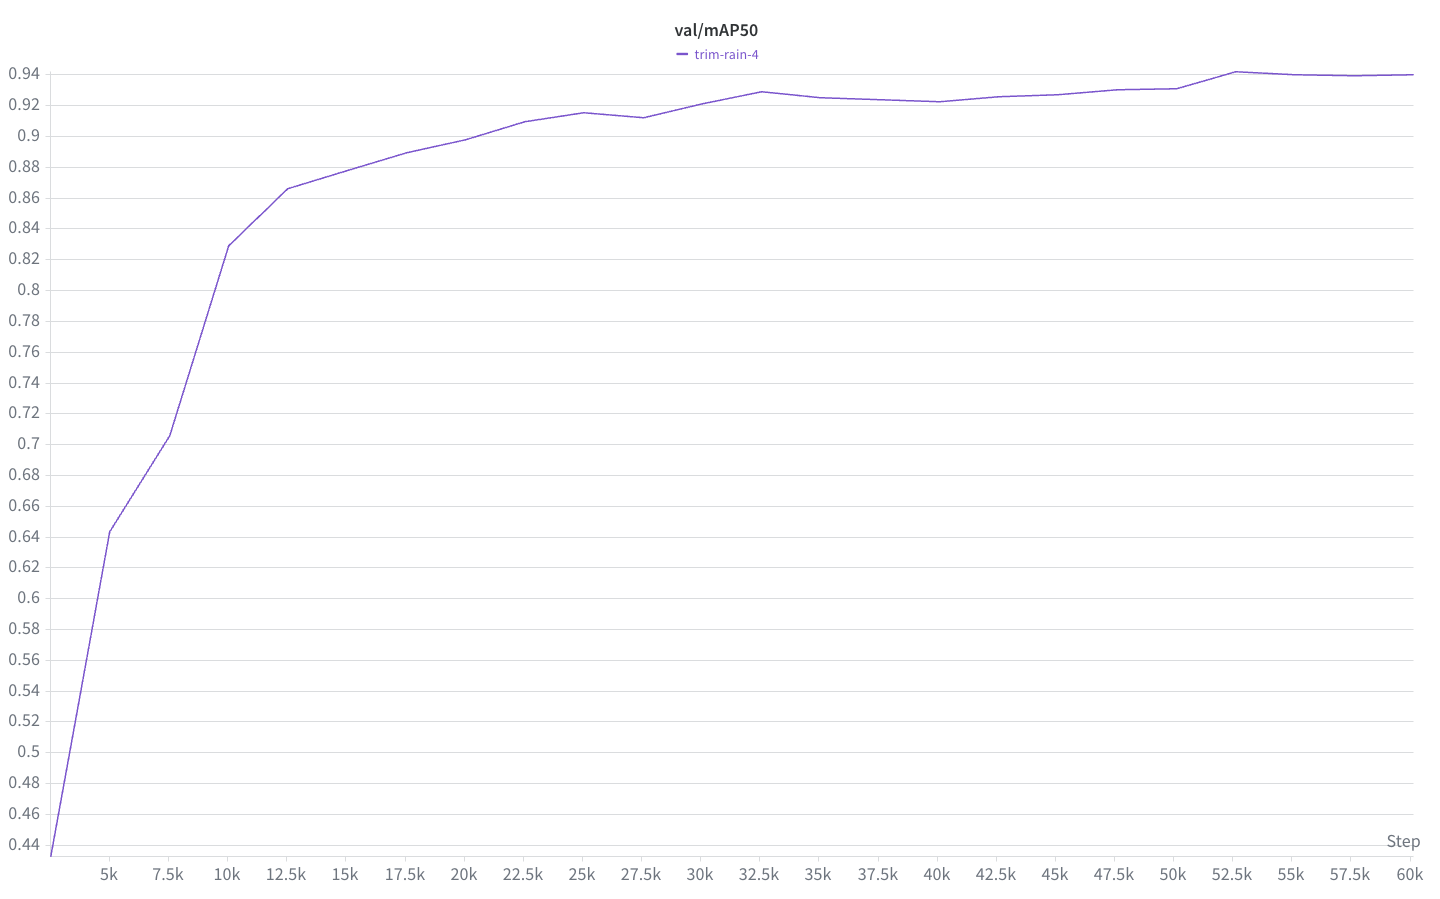
\includegraphics[width=\linewidth]{assets/val_map50.png}
  \caption{Validation mAP@0.5 over 24 epochs.}
  \label{fig:val_map50}
\end{figure}

\subsection{Per-Epoch Numbers}

\begin{table}[h]
  \centering
  \small
  \begin{tabular}{rccc}
    \toprule
    \textbf{Epoch} & \textbf{mAP} & \textbf{mAP$_{50}$} & \textbf{mAP$_{75}$} \\ \midrule
    0  & 0.1943 & 0.3888 & 0.1620 \\
    5  & 0.4367 & 0.8780 & 0.3556 \\
    11 & 0.4689 & 0.9217 & 0.3919 \\
    19 & 0.4668 & 0.9314 & 0.3875 \\
    20 (lr drop) & \textbf{0.4754} & \textbf{0.9422} & 0.4009 \\
    23 (final)   & 0.4726 & 0.9400 & 0.3988 \\
    \bottomrule
  \end{tabular}
  \caption{Per-epoch validation metrics. Peak occurs the epoch immediately after the StepLR drop at epoch 20.}
  \label{tab:per_epoch}
\end{table}

\subsection{Leaderboard}

\begin{figure}[h]
  \centering
  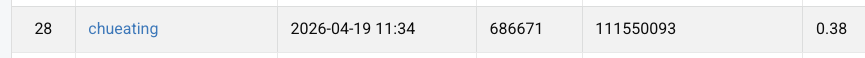
\includegraphics[width=\linewidth]{assets/leaderboard_screenshot.png}
  \caption{CodaBench public-leaderboard submission.}
  \label{fig:leaderboard}
\end{figure}

The final submission \texttt{pred.json} contains 49{,}979 detections covering all 13{,}068 test images, in the required COCO \texttt{[x,y,w,h]} (unnormalized, 1-indexed categories) format.

\subsection{Analysis}
The order-of-magnitude gap between mAP$_{50}$ (0.94) and mAP$_{75}$ (0.40) indicates that \emph{what} is detected is almost always correct but \emph{where} can be refined further---a known signature of DETR-family detectors with short training schedules. More decoder layers or a longer schedule would mainly tighten box localization. The lr-drop bump (\cref{tab:per_epoch}) confirms the 20/24 StepLR choice was near-optimal for this regime.

%------------------------------------------------------------------------

{\small
    \bibliographystyle{ieee_fullname}
    \bibliography{egbib}
}

\end{document}
